\documentclass[a4paper]{scrartcl}
\usepackage[utf8]{inputenc}
\usepackage[english]{babel}
\usepackage{graphicx}
\usepackage{lastpage}
\usepackage{pgf}
\usepackage{wrapfig}
\usepackage{fancyvrb}
\usepackage{fancyhdr}
\usepackage{float}
\usepackage{hyperref}
\pagestyle{fancy}

% Create header and footer
\headheight 27pt
\pagestyle{fancyplain}
\lhead{\footnotesize{Internet Applications, ID1354}}
\chead{\footnotesize{Name of the Report}}
\rhead{}
\lfoot{}
\cfoot{\thepage\ (\pageref{LastPage})}
\rfoot{}

% Create title page
\title{jQuery \& Ajax applications}
\subtitle{Internet Applications, ID1354}
\author{Linus Berg Linus@Fenix.me.uk}
\date{\today}

\begin{document}

\maketitle

\section{Introduction}

The seminar consisted of learning JavaScript, jQuery, and implement Ajax request
into the recipes website.
\section{Literature Study}
I was already familiar with jQuery and Ajax requests, all previous seminars
already utilised jQuery and Ajax.

\section{Method}
As stated above, all previous seminars utilised Ajax and jQuery, therefor no
changes were made for this seminar. However my initial thought during development
was that Ajax is a more modern method for updating a webpage rather than conducting
POST/GET requests by redirection, and I chose to implment it as I found it easier.
\\\\
\noindent
In the previous seminars, a simple .php file with a script was developed,
as can be seen in \href{https://github.com/linus-dev/KTH-Projects/tree/master/ID1354/2}{seminar 2},
then each one was easily requested via Ajax and a response was easily managed.
This separated the PHP from HTML further, and made the program easier to manage.
\\\\
\noindent
During \href{https://github.com/linus-dev/KTH-Projects/tree/master/ID1354/3}{seminar 3}, when
a MVC framework had to be implemented, the files were switched to the Laravel routing, and utilised
the controllers instead to manage each Ajax request.

\begin{center}
    \begin{tabular}{  l | r }
    Tool & Choice \\ 
    \hline
    Editor & \textit{Vim}\\
    Version Control & \textit{Git - Github}\\
    Web Server & \textit{nginx}\\
    Database & \textit{PostgreSQL 10.5-1}\\
    PHP & \textit{7.2.10-1} \\
    Framework & \textit{Laravel 5.7}\\
    \end{tabular}
\end{center}

\section{Result}
\href{https://github.com/linus-dev/KTH-Projects/tree/master/ID1354/4/laravel}{Github}
\\
As the javascript code was included since the first seminar the code has gone through
several structural changes in iterations, however, login has remained similar throughout
the program, with the addition of the CSRF token as can be seen in \ref{fig:auth}.
The login buttons have bound submit events via jQuery to submit an ajax request to the server
upon clicking one of the buttons, upon completion it reloads the site (this is obviously not
the way ajax was intended to be used, however the seminar did not mention you had to make
it rewrite the current page), this is because if the user was sucessfully logged in, the
page will reload and the laravel Auth model will display the logged in user instead.
\begin{figure}[H]
  \begin{center}
    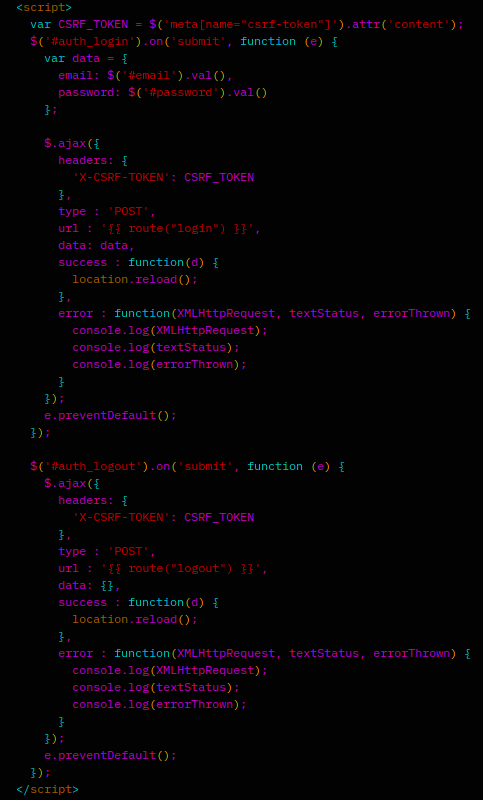
\includegraphics[scale=1.0]{images/login_out.png}
    \caption{Login and out.}
    \label{fig:auth}
  \end{center}
\end{figure}

\begin{figure}[H]
  \begin{center}
    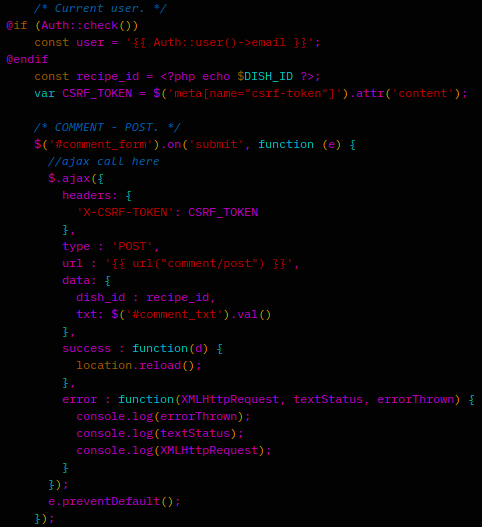
\includegraphics[scale=1.0]{images/post_cmt.png}
    \caption{Post comment.}
    \label{fig:post}
  \end{center}
\end{figure}
\noindent
Upon posting a comment the same as in the login buttons occur, a submit event is bound via jQuery
and upon triggering it submits an ajax request to the server with the relevant data to store the comment
in the database, again upon completion it reloads the current page.

\begin{figure}[H]
  \begin{center}
    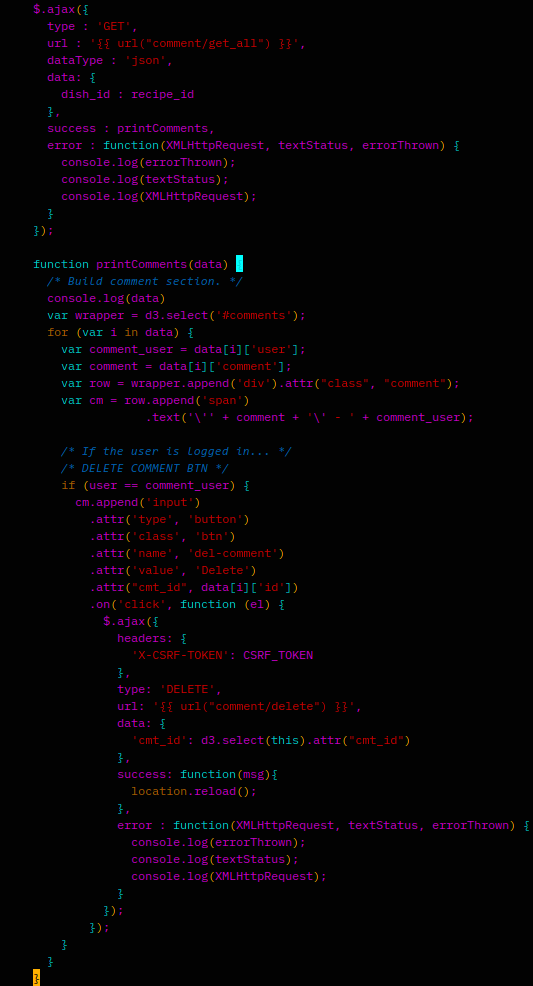
\includegraphics[scale=1.0]{images/build_cmt.png}
    \caption{Build comment section.}
    \label{fig:build}
  \end{center}
\end{figure}
\noindent
When the recipe page is loaded the scripts in \ref{fig:build} are executed,
creating a GET request to the server to recieve all comments for the relevant recipe,
in a json structure, no HTML data is sent,
this section could easily be modified to separate the printComments function so
the post comment code (\ref{fig:post}) does not need to reload the page.
\begin{figure}[H]
  \begin{center}
    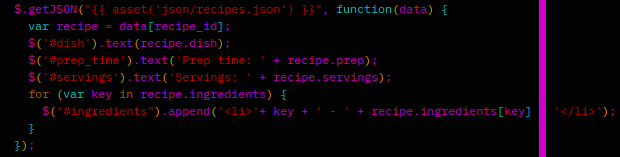
\includegraphics[scale=1.0]{images/build_recipe.png}
    \caption{Build recipe.}
    \label{fig:build_rec}
  \end{center}
\end{figure}
\noindent
Last but not least is the javascript to build the recipe description, prep time, and all the relevant information.
\ref{fig:build_rec} utilises the built in getJSON in jQuery, resulting in not needing to
set headers and manage data at a more rudimentary level.
\section{Discussion}

All the mandatory tasks have been met, ajax is used for almost every functionality on the site,
however not efficently as it still reloads the pages, this was more out of stress (I have to retake an exam Monday the 17th)
and I chose to not dwell too deep into the seminar to focus more on the exam.
\\\\
The javascript code could have been more structured as well, such as put into it's
own file and actually used classes, however it felt uneccessary for such
a simple task. Again javascript/jquery/ajax has been used since the first seminar, and some details were hard to recall
and I can not actually recall if any issues were encountered, however, I do not think there were any major problems.
In general it was hard to recall many details which is why the report is so sparse.
\end{document}
